%% LaTeX2e class for student theses
%% sections/evaluation.tex
%% 
%% Karlsruhe Institute of Technology
%% Institute for Program Structures and Data Organization
%% Chair for Software Design and Quality (SDQ)
%%
%% Dr.-Ing. Erik Burger
%% burger@kit.edu
%%
%% Version 1.3.3, 2018-04-17

\chapter{Evaluation}
\label{ch:evaluation}

The objective of our work is to provide a solution for the problem of exploration of large document collections.
To examine how well our proposed visualization meets the goal, an empirical evaluation is necessary.
This we achieve by conducting a summative user study, which is a part of the case study described in \autoref{ch:case_study}.
The purpose of this stage and the procedures for data collection have been decided upon as described in \autoref{subsec:procedures_for_data_collection}.
In this chapter we describe the execution of the summative study and discuss its results.

\section{Procedure}
\label{sec:procedure}

Four patent experts agreed to take part in the summative study.
Three of them had already participated in the formative study described in \autoref{sec:interviews}.

Being asked to perform tasks while being recorded might be stressful for the participants and therefore might influence the results negatively.
It is therefore recommended to preserve the context of the participants' usual workday routine as much as possible \cite{Portigal2013}.
For this reason, the study took place in a meeting room at the participants' workplace.
The participants were invited to solve tasks and talk about their experience while using the prototype in a one-on-one conversation.

Each individual appointment started with an explanation of the plan of the study: first a short introduction, then the first part focused on evaluating the usability of the prototype as a whole, followed by a second part focused on comparing the proposed approach with the baseline. 
The participants were encouraged to talk while they solved the tasks to describe what they were doing. 
The full plan of the study can be found in \autoref{sec:plan_summative_study}.

As a preparation for the actual study, two test rounds were conducted with volunteers with backgrounds outside the patent domain. 
This experience allowed us to experimentally detect inefficiencies and inconsistencies in the study plan and improve it before the proper study began.
The examiner had to multitask during the study:
\begin{itemize}
\item acknowledge the participants' statements and encourage them to think aloud
\item make sure that not too much time is spent on one task
\item look out for technical problems
\item guide the participants through the study procedure
\end{itemize}
For this reason, the practice rounds were immensely helpful to rehearse following the procedure of study plan exactly.

All four experts familiarized themselves with the ideas behind the visualization approach and with the prototype itself. 
This took place during the feedback meeting where the first proof-of-concept prototype was presented and also during the mid-term presentation for the thesis.
It allowed us to keep the introduction part short and to establish the rapport with the user quickly.

During the introduction, possible interactions with the prototype were explained and users were encouraged to try them out themselves immediately.
For that part, a dataset about 3D printers was used. 
This way, only the knowledge about how to control the prototype was transferable to the following tasks.

After the first task-solving part, a \gls{sus} questionnaire was offered. 
Some participants voluntarily commented on their answers.
Then a second task-solving part began.
With the study being in-subject, every participant evaluated both the semantic and the baseline approaches.
To counter learning effects, half of the participants tested the baseline approach first, then the semantic approach.
The other half started with the semantic approach first and finished with the baseline approach.

After the subject finished the tasks pertaining to one approach, a questionnaire was offered to capture impressions about that approach.
The participant was encouraged to speak about why they answered in the way they did.
The study ended with a brief general discussion of the participants' impressions, any perceived advantages and disadvantages of the prototype.
All relevant guidelines for the interviews already mentioned in \autoref{subsec:procedure} were followed: intentional pauses to encourage participants to speak, open questions instead of leading ones, etc.

Starting after the introduction, the study was recorded with the help of a screen capturing software OBS Studio.
The participants' actions and their commentary were captured and later transcribed for the evaluation.
The resulting script is 23 pages long and is not included in the thesis for brevity's sake and for the protection of the participants' privacy.
The transcription enabled us to make conclusions regarding the hypotheses we describe in \autoref{subsec:think_aloud}.

\section{Results}
\label{sec:results}

\subsection{Think-aloud}
\label{subsec:think_aloud}

We used the contact lens dataset described in \autoref{subsec:data_source} for the evaluation.
This domain was chosen partly because of the participants' background in chemistry and medicine.
Nevertheless, it is important to remember that the participants were not closely familiar with the subject of contact lenses.

We put forth a number of hypotheses to evaluate different aspects of the proposed approach.
The hypotheses from \autoref{subsubsec:hypothesis1} to \autoref{subsubsec:hypothesis5} pertain to usability of the prototype.
Evaluating them shows whether there is a match between the user interface and users' mental model of the patent landscaping task.
The last two hypotheses in \autoref{subsubsec:hypothesis6} and \autoref{subsubsec:hypothesis7} have the specific goal of comparing the baseline approach with the semantic approach.

\subsubsection{Hypothesis 1: Color mapping of points depending on sunburst is understood and helps identify clusters}
\label{subsubsec:hypothesis1}

Color is a pre-attentive visual attribute, which means differences in color are processed effortlessly and in parallel without any attention being focused on the display \cite{Treisman1985}.
Therefore, we expect that mapping categorical attributes, such as \gls{ipc} class, to colors helps experts identify coherent areas.

There were two tasks for evaluating this hypothesis:
\begin{itemize}
	\item Task 1. What \gls{ipc} classes (on the section level, one letter) appear together often?
	\item Task 11. Briefly describe broad thematic areas in the dataset (big clusters). Evaluate the positions of the clusters relative to each other.
\end{itemize}

\paragraph{During Task 1 the participants implicitly grouped same-colored points}~\\
Co-occurring \gls{ipc} classes yielded continuous areas with the same color combinations for both the semantic and the baseline approaches.
Assuming that the \gls{ipc} classes were assigned consistently, this indicates that both approaches were able to capture thematic groups within the domain.
All four participants referred to said continuous areas as opposed to single data points during their analysis for the task 1.
 
 \paragraph{Task 11 indicates that cluster boundaries are better understood when they differ in color}~\\
Task 11 needed to be solved twice per participant, once for each approach. 
The task 10 before task 11 required participants to switch to a single-colored representation.
They were asked to do so by choosing \textit{country} as a sunburst hierarchy because there was only one country present in the dataset.
It was anticipated that participants wish to switch back to the \textit{\gls{ipc} hierarchy} for the sunburst after completing the task.
Notably, one of four participants still stayed on a single-colored \textit{country} hierarchy kind.
It appears that they did not understand where exactly the boundaries of a labeled area lie.
They said ``There are areas not occupied with big key terms'' while they were describing areas on the largest cluster level.
In fact, due to the nature of agglomerative clustering, every data point always belongs to some cluster.
The area that was ``not labeled'' according to the participant's perception would have been the same color as the points around the nearest ``labeled'' area.
Conceivably, it would have been easier for the participant to identify boundaries of the cluster correctly if they had perceived one color within the cluster but different colors outside the cluster.

One participant had selected \textit{\gls{ipc} classes} as the sunburst hierarchy for both approaches.
While describing the areas, they circled with the mouse cursor around the boundaries of the clusters in a fairly precise way.
Other two participants had \textit{country} activated for one approach and \textit{\gls{ipc} classes} for another.
One of them circled around cluster boundaries on a colorful representation with \gls{ipc} classes, but not on a single-colored representation.
This might speak for the hypothesis.
The other participant moved the cursor from cluster label to cluster label, which is why it is impossible to estimate their perception of the cluster limits.

We anticipated that the participants would make a connection between the content of an \gls{ipc} class and cluster labels.
For example, one could expect reasoning analogous to the following: ``Areas with more blue points are overwhelmingly about chemistry, and the cluster about contact lens containers includes a group of blue points, so that means the containers  are probably treated with or hold some chemical solution.``
Unfortunately, no participant voiced any indication that they matched the labels of clusters with the content of the \gls{ipc} hierarchy.
It is nevertheless possible that they would have made this connection if they had been having the chance to work with the prototype for a longer time.
Participants themselves emphasized that they would normally spend significantly more time to familiarize themselves with the dataset, including the \gls{ipc} classes that are used within the data.

\paragraph{General observations}~\\
During the study, there were quite a few instances when colors within the scatter plot changed depending on what node was currently selected in the sunburst.
In every case, the mapping between colors and metadata values was directly obvious to the participants.
We therefore conclude that the dynamic color assignment was understood.

\paragraph{Summary}~\\
Ultimately, it was confirmed that the changing of the colors of the points depending on the sunburst state is understood. 
As for whether it helps identify the clusters, this part of the hypothesis is more likely to be confirmed than refuted.
Further experiments would be necessary to collect more evidence.

\subsubsection{Hypothesis 2: Glyphs as indication of co-occurrence of multiple values per metadata attribute are understandable and clearly visible}
\label{subsubsec:hypothesis2}

There were two tasks for evaluating this hypothesis:
\begin{itemize}
	\item Task 1. What \gls{ipc} classes (on the section level, one letter) appear together often?
	\item Task 3. Choose one of three largest assignees. Does this institution collaborate a lot with others? If yes, are they other institutions or individuals?
\end{itemize}

\paragraph{Co-occurence of \gls{ipc} classes}
\subparagraph{Intended solution}~\\
Our intended way of solving task 1 was to hover over each letter, one after another on the upper level of the \gls{ipc} hierarchy.
For each letter, the participants were supposed to roughly estimate how often the corresponding color appears on its own and with other colors.
One would also pay attention to the percentages in the breadcrumbs to support the estimation.
The expected conclusion would be that all patents belong to the class G - ``Physics'', while classes A, B and C are assigned to about a third of the patents each.
A majority of the patents belongs to two \gls{ipc} classes and a smaller number to three classes.
The most popular combination of two classes is G+A (red+green) occurring in 31\% of patents.

\subparagraph{Participants erroneously assume that choosing multiple sunburst nodes would show co-occurrences}
Two participants wrongly assumed that it was necessary to select multiple sunburst nodes simultaneously to display cooccurences.
One participant glanced to the keyboard which was intentionally placed out of reach. 
They searched for a way of selecting multiple nodes, such as clicking on them while holding a control key.
This erroneous attempt stemmed from the experience with desktop software where such mode of selection is popular, for example Windows Explorer or Microsoft Excel.
One participant also used the right-click hoping to find a suitable menu option in the context menu.

In web applications, right-clicking and using key combinations are not conventionally used.
From the above, we conclude that it was not immediately obvious to the participants that the prototype is a web application.
This conclusion is supported by the fact that participants were slightly confused when asked to refresh the web page when technical problems required a reset of the current state.

\subparagraph{Expert's perception of co-occurrence values was correct but occasionally incomplete}~\\
The first expert's initial impression was that G (red) occurs most often and that G+A (red+green) is the prevalent combination.
Then the participant examined color combinations by hovering the cursor over all one-letter \gls{ipc} classes one after another.
At the same time, they read percentage values in the breadcrumbs which confirmed their estimations.
They realized that 100\% the of data points belonged to \gls{ipc} class G  and guessed the reason for that correctly: ``It was probably used in the query to produce the dataset''.
The impression that red+green appears most often was also confirmed as the participant saw the value of 31\%.
All in all, this solution matched our expectations completely.

In addition to the first expert, one more participant was able to discover that 100\% of the data points belonged to \gls{ipc} class G - ``Physics''.
The remaining two experts nevertheless mentioned that the color of this class (red) occurs most often.
The total number of participants who saw the percentage values for classes A, B and C is two.
In the end, three experts were able to provide at least a partial solution for task 1.

One participant navigated into section A on the first level of the \gls{ipc} hierarchy and explained co-occurrences between subclasses of A, such as A61 and A45.
They however were unable to describe co-occurrences on the top level of the \gls{ipc} hierarchy when prompted, even though the course of action would be exactly the same and just the \gls{ipc} selection different.

\subparagraph{Colors in glyphs mix when seen from far away}~\\
In one case, the participant perceived purple color for glyphs composed of red and blue: ``On the first glance I thought it was purple and I could not find purple on the sunburst''.
We assume that the colors merged the same way blue, green and red diodes together can create a pixel of any color.
The effect did not apply any longer after the participant had zoomed in and glyphs had become slightly bigger, which supports our assumption.

\paragraph{Co-occurence of assignees}
\subparagraph{Intended solution}~\\
The expected procedure for solving this task would be to navigate into the chosen assignee node by clicking on it.
Then, the user would get an impression of how many points have just one single color corresponding to the selected assignee. 
If there were many multi-colored points that have multiple assignees, the participant would hover the mouse cursor over them and read the assignee entries in the detail view.
This way it would be possible to say if collaborators were mostly institutions or individuals.

\subparagraph{Experts' solutions}~\\
One participant understood \textit{cooperation} from the wording of the task not as co-occurrences of assignees, but as organizations citing each other's work.
As described in \autoref{subsubsec:forward_backward_citations}, this understanding is incorrect.
A citation purely indicates that the inventors are aware of existing inventions and still consider their patent novel.

All experts started the task by switching the sunburst hierarchy to \textit{assignees}. 
Despite the large number of assignees in the hierarchy, it was obvious to all users that assignees were ordered in the descending order by the number of applications.
One participant tried to detect co-occurrences by hovering over the tree top assignees in turn.
They were looking for points that stay visible after switching to another assignee.
In the end, all except one participant clicked the chosen assignee node, which happened to be Novartis AG in all cases, probably because it was the largest assignee. 
Then they hovered over multi-colored points and read the assignee information in the detail view for a number of patents.

One expert, however, did not realize that it was the intended way to solve the task: ``I can hover here and I get the assignee information, but it surely wasn't meant like this.''
They wished for a list of all assignees the chosen assignee has ever cooperated with.
According to them, only with such a list would they be able to see if the cooperations were mostly with organizations or individuals.

One more participant wished an alternative representation of assignee co-occurrences. 
They imagined a visualization in matrix form, possibly because they were familiar with such representation from the STN AnaVist software.
They also imagined a sunburst hierarchy \textit{assignee - assignee} in which the co-occurrences of assignees would be shown on the second level.
The idea would not be applicable to \gls{ipc} classes since it is not possible to display co-occurrences on different levels of \gls{ipc} hierarchy clearly in a way that is consistent with current interaction techniques for switching between levels.
Most importantly, in the current implementation of the sunburst child nodes indicate subgroups and not co-occurrences, which means that one would be introducing contradictions into the mental model of the sunburst control.

Ultimately, three experts were able to complete the task and answer the question.
Their conclusion was that Novartis AG does not cooperate much with other institutions.
When they do, it is mostly with individuals.
According to the experts, a characteristic feature of the US patent law is to enter the names of the inventors working for a company into the patent application as an assignee along with the the company itself.
Two experts explained that those individual assignees are most probably inventors working for Novartis AG.

\paragraph{Summary}~\\
Over the course of the two tasks, it has been confirmed that glyphs allow users to easily distinguish data points with one value of a categorical attribute from the points with multiple values.
When the goal is to provide a first impression about the distribution of values of metadata attributes, glyphs fit the purpose.
For a more detailed quantitative analysis of co-occurrences other representation forms are more suitable, for example, a co-occurrence matrix or a bar chart.

Furthermore, not using glyphs would mean that each data point would only be assigned one color.
Choosing to display only one value of a metadata attributes from a list of values would skew the perceived distribution of values because many values would not be displayed.
Considering all of the above, we consider the hypothesis confirmed.
Glyphs as they are used in our approach are an understandable indication of co-occurrence.
However, they are not sufficient for a detailed co-occurrence analysis.

\subsubsection{Hypothesis 3: The sunburst is suitable not only for hierarchical attributes, such as \gls{ipc} classes, but also for arbitrary sets of categorical attributes}
\label{subsubsec:hypothesis3}

The task for evaluating this hypothesis was Task 5: ``Compare in what \gls{ipc} areas \textit{Novartis AG} and \textit{Johnson \& Johnson Vision Care} are active''.

\paragraph{Intended solution}~\\
For this task, participants were expected to switch the sunburst hierarchy to \textit{assignees - \gls{ipc} codes}.
Then the anticipated course of action would be to navigate into the assignee node by clicking on it, examine the distribution of the \gls{ipc} classes, go back to the root of the hierarchy and do the same with the other assignee.

\paragraph{Switching the sunburst hierarchy kind}~\\
The previous task left the sunburst hierarchy set to \textit{assignees} and all participants understood the need to switch hierarchy kind.
This was the first time the participants needed to use two metadata attributes simultaneously in the sunburst.
One participant first navigated to Novartis AG on the assignee level, then attempted to change the hierarchy to \textit{\gls{ipc} classes}, which brought invalid results due to a technical problem.
Apparently, they expected that the currently selected hierarchy node persists after switching to another kind of hierarchy.
After they realized their misconception, they were able to choose the expected hierarchy kind successfully.

\paragraph{Navigation was problematic because of performance issues}~\\
Participants had a reliable grasp on navigation between the levels of the sunburst.
All of them realized the need to navigate into a node if its child nodes are currently too small for convenient interaction.

The assignees mentioned in the task are ones in the top three according to the total number of patent applications.
This is intentional because of the large number of assignees in the dataset (about 1100).
Measures were taken to merge assignees with different spellings into one entry as described in \autoref{subsec:data_preprocessing} ``Parsing of metadata attributes''.
However, the resulting view still permitted working comfortably with approximately top 20 assignees only.
The rest of the assignees occupied a sector of the circle too small to be selected reliably with the mouse.

As is, using assignees as the first level of the sunburst hierarchy resulted in a suboptimal experience for the participants because of performance problems.
For some participants, it took time to learn to wait until the hover or click interactions were completely rendered by the prototype.
When they did not immediately see the result of their actions, they moved the mouse cursor around and accidentally hovered over small assignees they did not recognize.
After participants learned what response times to expect, all of them were able to successfully navigate to an assignee of choice and back to the root of the hierarchy.
One expert said: ``I thought you could type it in here somewhere'' referring to the choice of an assignee.

\paragraph{Summary}~\\
All experts were able to describe the differences in the distribution of \gls{ipc} classes for two chosen assignees.
They compared the size of the same sunburst nodes not only on section level (e. g. G), but on the class level (e. g. G02) as well.
One expert stated that the differences ``can be seen well''.

One conceivable solution to the challenge of showing many nodes on the same hierarchy level would be to enlarge the sunburst control to fit the whole screen. 
For hover interactions to be possible while still seeing the data points, one would move the enlarged sunburst control to a second monitor.
An alternative solution would be to only distinguish between the top 10 to 20 assignees and aggregate the rest into the category ``Others''.
The disadvantage of this approach is that it would be difficult to perceive the distribution of assignees by the number of applications, i. e. whether the technology domain is dominated by a few powerful companies or many smaller ones.

Until a solution is implemented, we would discourage from using the sunburst chart for metadata attributes with tens of different values.
For the patent landscaping scenario, country and \gls{ipc} class are attributes that result in a clear usable representation in a sunburst, while assignee is not suitable.
The hypothesis is therefore considered partly confirmed.

\subsubsection{Hypothesis 4: The interaction of all parts of the interface is understood}
\label{subsubsec:hypothesis4}

There were two tasks that could only be solved if the interaction between the sunburst view and the histogram view was clearly understood by the participant:
\begin{itemize}
	\item Task 2. During what timespan does the \gls{ipc} area G02C13 (Assembling; Repairing; Cleaning) actively develop?
	\item Task 4. Compare the timelines of applications for the assignees \textit{Johnson \& Johnson Vision Care} and \textit{Bausch \& Lomb}.
\end{itemize}
Furthermore, no view in the interface is so independent from the others that it could provide full benefits if taken alone.
This means the remaining tasks also significantly contributed to the testing of this hypothesis.

\paragraph{Trends in development of an \gls{ipc} class}
\subparagraph{Intended solution}~\\
This task was intended to be completed as following. 
First, the sunburst hierarchy has to be switched to ``\gls{ipc} classes''.
Second, one needs to interact with the node that represents G02C13 either by hovering over it or by clicking on it.
In case of hovering, the number of applications for this subclass will be overlaid over the histogram view in the matching color.
In case of clicking, only applications in this subclass will be shown in the histogram view.
The participant would then be able to detect application peaks, time intervals with a significant number of applications and with little to no applications.

\subparagraph{Interaction between sunburst and histogram is clear}~\\
All four participants preferred clicking on G02C13 instead of hovering over it.
We suppose that clicking is a more widespread and intuitive interaction form than hovering and therefore participants were more comfortable with clicking.
Importantly, every expert connected the change in the values of the histogram to their previous action of selecting the subclass.
Accordingly, all four were able to describe the trend of G02C13's development.
The years they named as a period of active development were consistent between participants.

\paragraph{Trends in development of an assignee}
\subparagraph{Participants' solutions}~\\
The solution of task 4 was very similar to the one of task 2, except the participants should change the sunburst hierarchy kind to \textit{assignee}.

As described in the previous paragraph, during task 2 no participant has intentionally used the hover interaction on a sunburst node to see the number of applications per year for that node.
Notably, by task 4 two of the participants became accustomed to the hover interaction and successfully used it to solve the task.

One participant navigated into the required assignee node, then back up and to the second assignee.
While doing so, they expressed some frustration about not being able to see the timelines for both assignees at the same time: ``One cannot remember all of this''.
They intended to perform a thorough year-per-year comparison, which is more effort than the task actually required.

In fact, this is where the advantage of the hover interaction becomes apparent as compared to clicking into the assignee node.
Going one level back to switch to another assignee requires a change of context.
A hover interaction, however, takes place at the root level of the sunburst hierarchy and does not require switching back and forth.
It also takes less time so it is easier to keep the values of the time-series in short-term memory.
Nevertheless, we agree that for detailed quantitative comparison it is necessary to display both time series simultaneously.

\subparagraph{Interaction between sunburst and histogram is clear and adds value}~\\
In the end, all experts were able to complete the task.
After they saw no new applications for Bausch \& Lomb since 2009, one participant was able to put this fact in the context of their domain knowledge: ``it stops then because the company does not exist anymore''.
One participant said that ``it is often interesting to see this'' referring to the evolution of the domain through the years.
Another participant agreed that it was ``by all means'' useful to be able to examine the time dimension.

Tasks 2 and 4 allow us to confirm that the interdependence between the sunburst nodes and the time series values in histogram view was indeed clear to the participants.
Our visualization approach is thus considered suitable for the \textit{trend analysis} usage scenario.\todo{refer to scenarios}

\paragraph{Interactions between the sunburst itself and the breadcrumbs}~\\
It is impossible to say exactly how the breadcrumbs view was utilized without a camera or an eye-tracking system which we did not use.
Nevertheless, reading can be recognized when the person whispers the words or says them aloud, or when the person moves the mouse to the text they are reading.
It is especially interesting to know whether the experts took advantage of the full descriptions for the \gls{ipc} classes and unshortened assignee names.

We can say confidently that the changes in the breadcrumbs view depending on the the actions in the sunburst were clear to all participants.
For example, if they navigated into a sunburst node, they were reassured of the result of their action because the navigation path was shown with the breadcrumbs.
Notably, for tasks involving \gls{ipc} classes, the participants often read the descriptions for the upper level of the \gls{ipc} hierarchy, but seldom for deeper levels.
We attribute this to the fact that the experts were not familiar with the domain of contact lenses.
They probably did not see the point in getting acquainted with the \gls{ipc} classes from this domain, especially considering the short-term nature of the tasks in the study.

Providing the descriptions for \gls{ipc} classes implements the principle of \textit{recognition instead of recall} as described in \autoref{subsubsec:breadcrumbs}.
The experts can easily browse through the nodes in the sunburst and recognize the thematic areas they search for.
This feature was also requested by the experts during the feedback meeting when the first iteration of the prototype was presented.
Therefore, textual content along with the graphic breadcrumb nodes provides added value.
For the above-mentioned reasons, we are convinced that the visual metaphor for the breadcrumbs view is chosen appropriately.

\paragraph{Interactions involving scatter plot and detail view}~\\
Task 3 (assignee co-occurrences, see \autoref{subsubsec:hypothesis2}) and all tasks from part 2 of the evaluation relied on information only visible in the detail view.
Except for cases of overlapping points (see \autoref{subsubsec:hypothesis5}) or points obscured by cluster labels, the participants were able to retrieve detailed information for a chosen point confidently.

As with hover vs. click interaction on the sunburst (see the beginning of this subsection), some participants were initially more comfortable with clicking, even when they did not need the information in the detail view to persist (e. g. for comparison).

\paragraph{Summary}~\\
Summing it up, the participants grasped the interplay between sunburst and histogram, sunburst and scatter plot (see \autoref{subsubsec:hypothesis1}), scatter plot and detail view (see above).
Notably, the training in the beginning of the study only took 10 minutes.
After the training the experts were able to reliably control the visualization.
We therefore consider the hypothesis confirmed. 

\subsubsection{Hypothesis 5: Dynamic density of labels for points and clusters results in a readable and informative presentation}
\label{subsubsec:hypothesis5}

Intended for evaluating this hypothesis was task 6: ``Navigate into the dataset with panning, zooming in and back out and assess the readability of labels in different levels of detail''. 
The task is self-explanatory.

One participant asked why a point had no label while they were on a middle detail level.
As described in \autoref{subsubsec:points} ``Zooming'', adaptive density of labels was implemented for readability reasons.
This fact, however, was not included into the introduction to the study for brevity's sake.

Participants described the point labels as well-readable with just one exception.
When the scatter plot was zoomed in to the maximal detail level (zoom factor 10), the top three relevant terms were shown per patent.
In some cases the points were situated close enough for the labels to overlap and become unreadable.
This happens when points are approximately at the same position horizontally and the labels are long.
According to one expert, if two points are so close that they overlap, ``it is even more important to know what the differences [between them] are''.
The expert hoped to comprehend the difference based on the top three key terms.

The participants asked for the overlapping problem to be solved and suggested solutions themselves. 
For example, they suggested automatically moving overlapping points away from each other at the maximal zoom level.
One participant asked if they could ``play around'' with overlapping points, with the intention to pull them apart.
Allowing users to manually move points would be a simple alternative to an automatic overlap removal algorithm.
Another simple solution that takes almost no implementation effort would be just increasing the maximal allowed zoom level so that points stand further apart.
One more alternative suggested by an expert is to bring a point into foreground when it is hovered over. 
For this idea to work as intended, a contrast background has to be added behind the active point to separate it from its neighbors and make the label readable.

\paragraph{Summary}~\\
No participants perceived that there were too many or too few labeled points, which is exactly the result we were aiming for with the heuristic for a proportion of shown labels.

Our observation did not reveal any readability problems except the mentioned overlapping issue.
The hypothesis is considered confirmed.

\subsubsection{Hypothesis 6: Cluster labels computed based on word2vec-based embeddings correspond to human understanding in a better way than those in TF-IDF-based embeddings}
\label{subsubsec:hypothesis6}

The task specifically aimed at evaluating this hypothesis was Task 11: ``Briefly describe broad thematic areas in the dataset (big clusters). Evaluate the positions of the clusters relative to each other''.
This task is very reliant on the significance of cluster labels.
Most importantly, all tasks from part two of the study implicitly assess this hypothesis.

% Table generated by Excel2LaTeX from sheet 'Sheet1'
\begin{longtable}[htbp]{|r|p{11.3em}|p{11.3em}|p{10em}|}
  \caption{Comparison of cluster key terms for both approaches. Contact lens dataset}\\
   \toprule
   \multicolumn{1}{|c|}{\multirow{2}[4]{*}{\textnumero}} & \multicolumn{2}{c|}{Top 15 key terms per approach} & \multirow{2}[4]{*}{Experts' description} \\
   \cmidrule{2-3}      & Semantic & Baseline & \multicolumn{1}{c|}{} \\
   \midrule
    \endhead
    \multicolumn{4}{r}{\textit{Continued on next page}} \\
    \endfoot
    \bottomrule
    \endlastfoot
    \midrule
    1 & \textbf{enzyme}, \textbf{cleaning}, \textbf{disinfecting}, \textbf{polyionic}, \textbf{polyionic material}, \textbf{salt}, \textbf{peroxide}, \textbf{surfactant}, \textbf{composition}, hydrogen peroxide, \textbf{polyoxyethylene}, \textbf{deposits}, \textbf{antimicrobial}, \textbf{polyanionic}, aqueous medium & \textbf{cleaning}, \textbf{polyionic}, \textbf{enzyme}, \textbf{surfactant}, \textbf{disinfecting}, \textbf{polyionic} \textbf{material}, medical device, \textbf{polyanionic}, medical, \textbf{composition}, \textbf{salt}, \textbf{antimicrobial}, \textbf{polyoxyethylene}, \textbf{peroxide}, \textbf{deposits} & -Cleaning\newline{}-Enzymes, cleaning, hygiene, disinfection\newline{}-Cleaning, disinfection\newline{}-Enzymes for cleaning of lenses\newline{}-Cleaning systems\\
    \midrule
    2 & \textbf{prepolymer}, \textbf{divalent} \textbf{radical}, methylene pyrrolidone, macromonomer, \textbf{divalent}, \textbf{crosslinkable}, \textbf{vinylic}, \textbf{crosslinker}, \textbf{alk}, meth, parts weight, \textbf{hydrocarbon}, \textbf{denotes}, \textbf{compound}, polymerizable composition & \textbf{crosslinkable}, \textbf{prepolymer}, \textbf{compound}, \textbf{divalent} \textbf{radical}, \textbf{divalent}, \textbf{alk}, binder, radical carbon, \textbf{hydrocarbon}, \textbf{denotes}, \textbf{vinylic}, vinylic monomer, ink, binder polymer, \textbf{crosslinker} & -Materials the lens consists of, they are polymers\newline{}-Materials\newline{}-What the lens consists of\newline{}-Substances, polymers the lens consists of\newline{}-How the materials are produced \\
    \midrule
    3 & medical device, dye, medical, ink, article, \textbf{precursor}, \textbf{polymeric} \textbf{material}, reactive, \textbf{hybrid}, ophthalmic lens, cellulose, \textbf{hybrid} \textbf{contact}, \textbf{polymerizable} \textbf{composition}, anti, printing & \textbf{hybrid}, \textbf{polymerizable} \textbf{composition}, \textbf{hybrid} \textbf{contact}, \textbf{polymeric} \textbf{material}, \textbf{precursor}, siloxane monomer, collagen, core, aromatic, aromatic based, extracted, polymeric lens, macromer, rigid, composite &-Materials the lens consists of\newline{}-Materials\newline{}-Lens itself, its shape\newline{}-Colorants\newline{}-Products \\
    \midrule
    4 & \textbf{central} \textbf{zone}, \textbf{aberration}, \textbf{meridian}, \textbf{optical} \textbf{zone}, \textbf{vertical} \textbf{meridian}, \textbf{refractive} \textbf{power}, \textbf{central} \textbf{optical}, \textbf{model}, \textbf{inferior}, \textbf{spherical} \textbf{aberration}, \textbf{optic} \textbf{zone}, \textbf{segment}, \textbf{stabilization}, \textbf{lens} \textbf{design}, transition zone & \textbf{central} \textbf{zone}, \textbf{aberration}, \textbf{meridian}, \textbf{optical} \textbf{zone}, \textbf{refractive} \textbf{power}, \textbf{vertical} \textbf{meridian}, \textbf{central} \textbf{optical}, \textbf{model}, \textbf{optic} \textbf{zone}, \textbf{inferior}, multifocal contact, \textbf{spherical} \textbf{aberration}, \textbf{segment}, \textbf{lens} \textbf{design}, \textbf{stabilization} & -Optical power. When someone has astigmatism, how the lens should be bent, its form\newline{}-Abberation is how you see\newline{}-Vision corrections as known from an optician \\
    \midrule
    5 & \textbf{container}, \textbf{chamber}, \textbf{package}, \textbf{housing}, \textbf{cleaning}, \textbf{lens} \textbf{package}, \textbf{reservoir}, \textbf{holder}, \textbf{cap}, \textbf{lens} \textbf{holder}, \textbf{cup}, \textbf{lens} \textbf{cleaning}, shaft, insert, carrier & \textbf{container}, \textbf{chamber}, \textbf{package}, \textbf{housing}, \textbf{cleaning}, \textbf{lens} \textbf{package}, \textbf{holder}, \textbf{cap}, \textbf{reservoir}, mold part, \textbf{lens} \textbf{holder}, station, \textbf{lens} \textbf{cleaning}, \textbf{cup}, male & -Containers \newline{}-Packaging\newline{}-Where the lenses are stored\newline{}-How packaging is, how lenses are stored, reservoirs etc. \\
    \midrule
    6 & \textbf{iris} \textbf{section}, \textbf{iris}, \textbf{shade}, \textbf{color}, \textbf{limbal} \textbf{ring}, \textbf{starburst}, \textbf{limbal}, \textbf{colored}, \textbf{dots}, \textbf{cosmetic}, \textbf{colorant}, white, ophthalmic lens, beam, \textbf{colored} \textbf{contact} & \textbf{iris}, \textbf{iris} \textbf{section}, \textbf{shade}, \textbf{colorant}, pattern, \textbf{colored}, \textbf{cosmetic}, \textbf{limbal} \textbf{ring}, \textbf{color}, \textbf{starburst}, \textbf{limbal}, \textbf{colored} \textbf{contact}, \textbf{dots}, dot, indicator & -Colored lenses\newline{}-How the iris is built\newline{}-The eye, the iris as an organ \\
    \midrule
    7 & \textbf{substrate}, \textbf{signal}, \textbf{sensing}, \textbf{information}, \textbf{antenna}, circuit, sensors, circuitry, \textbf{data}, wireless, disposed substrate, \textbf{energy}, reader, electrodes, \textbf{ophthalmic} \textbf{device} & \textbf{ophthalmic} \textbf{device}, \textbf{substrate}, \textbf{energy}, \textbf{signal}, dynamic, beam, ophthalmic lens, \textbf{data}, \textbf{information}, \textbf{sensing}, insert, filter, display, \textbf{antenna}, reflected & -Not clear\newline{}-Some physical methods\newline{}-Antennas, circuits, sensors. Those are devices that measure properties of lenses\newline{}-Sensors, measuring devices\newline{}-The end product (device), but also electronical properties, energy \\
  \label{tab:comparison_clusters}%
\end{longtable}%

For both semantic and baseline (\gls{tf-idf}-based) approaches, the top level of hierarchical clustering consisted of 7 clusters.
\autoref{tab:comparison_clusters} shows cluster terms for both approaches and the way the experts described the content of the corresponding area (see \autoref{subsec:hierarchical_clustering} for details on key term extraction).
For 5 out of those 7 clusters (clusters \textnumero1, \textnumero2, \textnumero4, \textnumero5, \textnumero6), the key terms were very similar between the approaches.
In fact, at least two of the top three terms were exactly the same for both approaches.
In case of clusters \textnumero4, \textnumero5 and \textnumero6 even all three terms were the same.

\paragraph{Experts were often able to consistently identify same areas between different approaches}~\\
Predictably, after the participants identified and described large thematic areas for one approach, they were able to instantly recognize comparable areas for another approach.
The experts' descriptions of those areas were consistent:
\begin{itemize}
\item Cluster \textnumero1 is about cleaning of contact lenses with enzymes.
\item Cluster \textnumero2 contains materials contact lenses are made of.
\item Cluster \textnumero4 is about optical properties of the lenses and how they assist vision correction.
\item Cluster \textnumero5 describes the storage of lenses in suitable containers.
\item Cluster \textnumero6 is about colored contact lenses, according to three experts. One expert was led astray by the term ``iris'' as they assumed it could only refer to the organ. Human body parts, however, are not patentable by themselves. In this case, the iris is discussed in the context of a colored contact lens. An artificial pattern on the lens covers the iris and sometimes tries to replicate the aesthetics of a real iris.
\end{itemize}

In contrast to the abovementioned five clusters, the two remaining ones (clusters \textnumero3, \textnumero7) lead to most incoherent descriptions.
Cluster \textnumero3 includes fairly inhomogenious topics, which resulted in the top three terms being completely different between the approaches (medical device, dye, medical vs. hybrid, polymerizable composition, hybrid contact).

``Medical'' is, in context of contact lenses, a very general term that did not contribute much to the understanding of the domain.
The participants struggled with its interpretation during the evaluation of the semantic approach.
By contrast, chemical terms from the baseline approach were specific enough for a better understanding.
For both approaches, the cluster \textnumero2 labeled by additional chemical terminology (crosslinkable, prepolymer, compound) was very close to the cluster \textnumero3 and partly merged with it.
Because of that, for the baseline approach some participants described both clusters \textnumero2 and \textnumero3 together as containing materials for producing contact lenses.

Experts appeared to have difficulties describing cluster \textnumero7 because they were not very familiar with the domain of electronics, in particular wearables.
The term ``substrate'' in this case refers to the material the electronic circuits are placed upon .
Most participants have a background in chemistry, where substrate refers to the chemical of interest that is being modified \cite{mcnaught1997compendium}.
It is possible that the discrepancy in the understanding of this term led to some confusion.
In the end, no expert described this area sufficiently well.

\paragraph{Relative importance of top key terms}~\\
The participants' ideas about the content of the clusters seemed to be influenced greatly by the top three terms per cluster that are always visible.
After an initial assumption about the topic of the cluster was made, the remaining 12 of 15 top terms (shown on mouseover) seemed not to alter the first idea.
This might be explained by the perceptual principles of the visual hierarchy.

Objectively speaking, the fourth top term does not differ much in relevance compared to the third top term.
In fact, all 15 top terms enhance each other well and provide meaning for the user when considered together.
However, the fourth and further key terms are only visible on demand, and are shown in a much smaller font size.
Those are the trade-offs that we chose to make for the sake of readability.
It is likely that because of that, the perceived relevance of the fourth and further top terms is much lower, and they are not taken into account by the experts as much.

If we were to increase the font size of the on-demand terms to match the top three, we would have to distribute them around the cluster to avoid overlaps and visual clutter. 
Depending on the length, some terms might even land outside the cluster boundaries.
All of this would suggest to the users that the exact position of the terms inside a cluster matters, which is not the case here.
A better solution remains to be found.

\paragraph{Experts' perceptions of key terms}~\\
Regarding the key terms themselves the experts had varied opinions.
One participant struggled to see the added value in the extracted terms.
According to them, there were many irrelevant terms among the ones extracted for clusters and single patents.
They explained that, for example, ``pharmaceutical composition'' is a very common phrase in the domain of medicine, and ``bottom portion'' or ``side walls'' are used ubiquitously when describing devices of any kind.

We agree that such phrases have little explanatory power, but only in the case of a homogeneous dataset where every patent is about medicine or about devices, accordingly.
In our case, however, the contact lens dataset contained a diverse range of topics.
The example phrases mentioned by the expert really can make the difference between different thematic areas visible.
It is quite possible that for a less diverse dataset, such terms would not be considered ``relevant'' by the \gls{tf-idf} algorithm. 
Since they appear in the most patents within the corpus, the \gls{idf} would lower their computed relevance.
A more extensive stopword list can nevertheless be of great help for the quality of extracted terms.

Notably, we used \gls{tf-idf} as a baseline approach for the key term extraction for single patents (the approach for clusters is described in \autoref{subsec:hierarchical_clustering}).
We experimented with the algorithm's parameters, but the potential for improvement is not exhausted yet.
Moreover, a number of more advanced algorithms based on \gls{tf-idf} exist \cite{Liu2010} \cite{Kim2009}.
So do key term extraction methods not based on \gls{tf-idf} like \gls{rake} \cite{rose} and TextRank \cite{Mihalcea2004}.
It might be beneficial to test the above-mentioned algorithms on patent texts.

The expert mentioned above was also wondering about the differences between adjacent points with disparate key terms: ``To really analyze this, I need to know why those two are so close, and why are the extracted terms then so different?''
We strongly agree with the requirement for explainability.
In this case, however, the interpretation is made difficult by the fact that we are observing a space after the dimensionality reduction.
One conceivable reason for dissimilar terms for supposedly semantically close documents might be a lot of shared vocabulary, which nevertheless does not show up in extracted terms as it is too widespread within the document corpus.
This leaves the most narrowly used terms to be extracted as relevant.

Overall, the experts' perception was that the key terms are more useful for bigger clusters, where they also describe more general concepts: ``On the higher levels the terminology is more helpful, so that you can associate it with something''.
The key terms become less helpful as one focuses on the specifics of a small group of documents.
Nevertheless, one expert found multiple levels of detail for hierarchical clustering a helpful feature: ``it has the generated terminology on two [sic] different levels, this is good''.

\paragraph{Suggestions for improvements}~\\
The above-mentioned participant was also happy to see the areas labeled at all because ``in other software you have to write the titles yourself''.
To give users the ability to compose their own captions for arbitrary areas is a feature that was already mentioned by the experts during the mid-term presentation of the thesis.
It would be immensely helpful for a detailed analysis to be able to draw a boundary around an interesting area.
This would follow the principle of \textit{recognition over recall}.
It is a user interface design pattern that requires significantly less cognitive effort from the user when implemented.
In this case, it takes less mental effort for the user to process an area they labeled themselves versus when they are forced to recollect their description of the area every time.
Should our prototype be developed further as a product, this is a functionality that might be worth implementing.

All participants wished for a search functionality based on document terms when confronted with tasks that required zooming into the landscape: ``it is difficult. I have this information [from the task] and I can't search, but can only zoom, hover and read''.
They would expect to see highlighted areas where the queried term appears often: ``it would show me where it [the requested term] is and jump there. Maybe one [document] will be here and one there. It would say, here on the upper-left side there is a hotspot''.

One participant had an impression that the baseline approach resulted in better key terms for the clusters, but could not elaborate on their vague feeling.

\paragraph{Cluster terms overlap significantly between approaches}~\\
To examine whether the similarity of cluster terms between both approaches is pertinent only to the contact lens dataset, we compared the top 15 terms for other datasets used in this thesis: 3d printers, video codecs, hair dryers and diesel engines. 
In the overwhelming majority of the cases, we could determine a one-to-one correspondence between clusters for both approaches based on common themes suggested by overlapping key terms. 
The results can be seen in \autoref{sec:term_comparison} with the identical terms emphasized in bold.

It can easily be seen that a greater part of cluster key terms are exactly the same.
The hair dryer dataset is the one where the corresponding clusters were most difficult to define.
We attribute this to a small sample size (ca. 350 documents), where influence of noise and of individual properties of the algorithms is unlikely to be compensated.
In fact, the number of matching terms among the top 15 terms per cluster increases with the size of the dataset.
Clearly, matching terms can only be a result of a term extraction on approximately the same subset of the data.
This shows that both semantic and baseline approaches group the same patents in a similar way, at least at the most general level.

Considering all of the above, with regard to key terms none of the compared approaches provided a significant advantage over the other.
The hypothesis is therefore refuted.

\subsubsection{Hypothesis 7: Distances between points in word2vec-based embeddings correspond to human understanding in a better way than those in TF-IDF-based embeddings}
\label{subsubsec:hypothesis7}

In the same way as with \autoref{subsubsec:hypothesis6}, all tasks from part 2 of the study are applicable to evaluate this hypothesis:
\begin{itemize}
\item Task 7. Find the area/areas with patents about colored contact lenses.
\item Task 8. Find the area/areas with patents about contact lenses with electronic components (“smart” contact lenses)
\item Task 9. Find the area/areas with patents about cleaning of contact lenses.
\item Task 10. Find the area/areas with patents about ordering systems for contact lenses. They handle interaction with the client: diagnosis, ordering of lenses for example as a subscription, adjusting the prescription, etc.
\item Task 11. Briefly describe broad thematic areas in the dataset (big clusters). Evaluate the positions of the clusters relative to each other.
\end{itemize}

\paragraph{Searching for large areas}~\\
Tasks 7 and 9 were designed to be solved in a similar way for comparability, with one task per approach.
For those tasks, we wanted to evaluate the approaches independently of the patent's metadata, only based on the textual content.
For that, the participants were asked to choose ``Country'' as a hierarchy level for the sunburst.
The dataset consisted of only patents from the US patent office, so filtering and highlighting features were not accessible for that single value.

\subparagraph{Our examination of relative cluster placement}~\\
Both colored contact lenses and cleaning of contact lenses comprise their own large clusters (see clusters \textnumero6 and \textnumero1 in \autoref{tab:comparison_clusters}).
Additionally, there are significant areas with related patents within other clusters.
in \autoref{fig:colored_ink}, we highlight the main large cluster of interest, the smaller relevant areas and the bigger cluster they are a part of.

\begin{figure}[!]
    \centering
    \subfigure[Semantic approach]
    {
	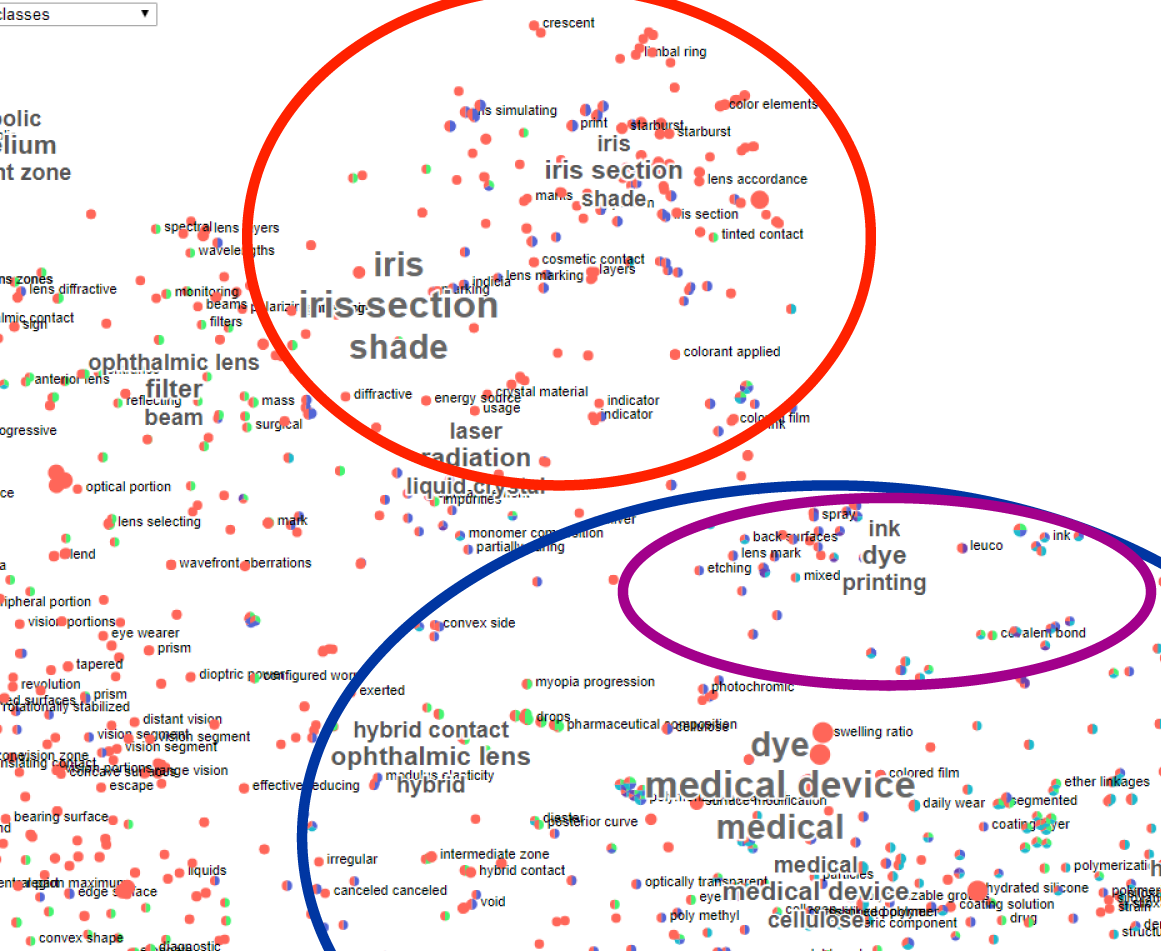
\includegraphics[width=\textwidth]{img/colored_ink_semantic}
        \label{fig:colored_ink_semantic}
    }\\
    \subfigure[Baseline approach]
    {
        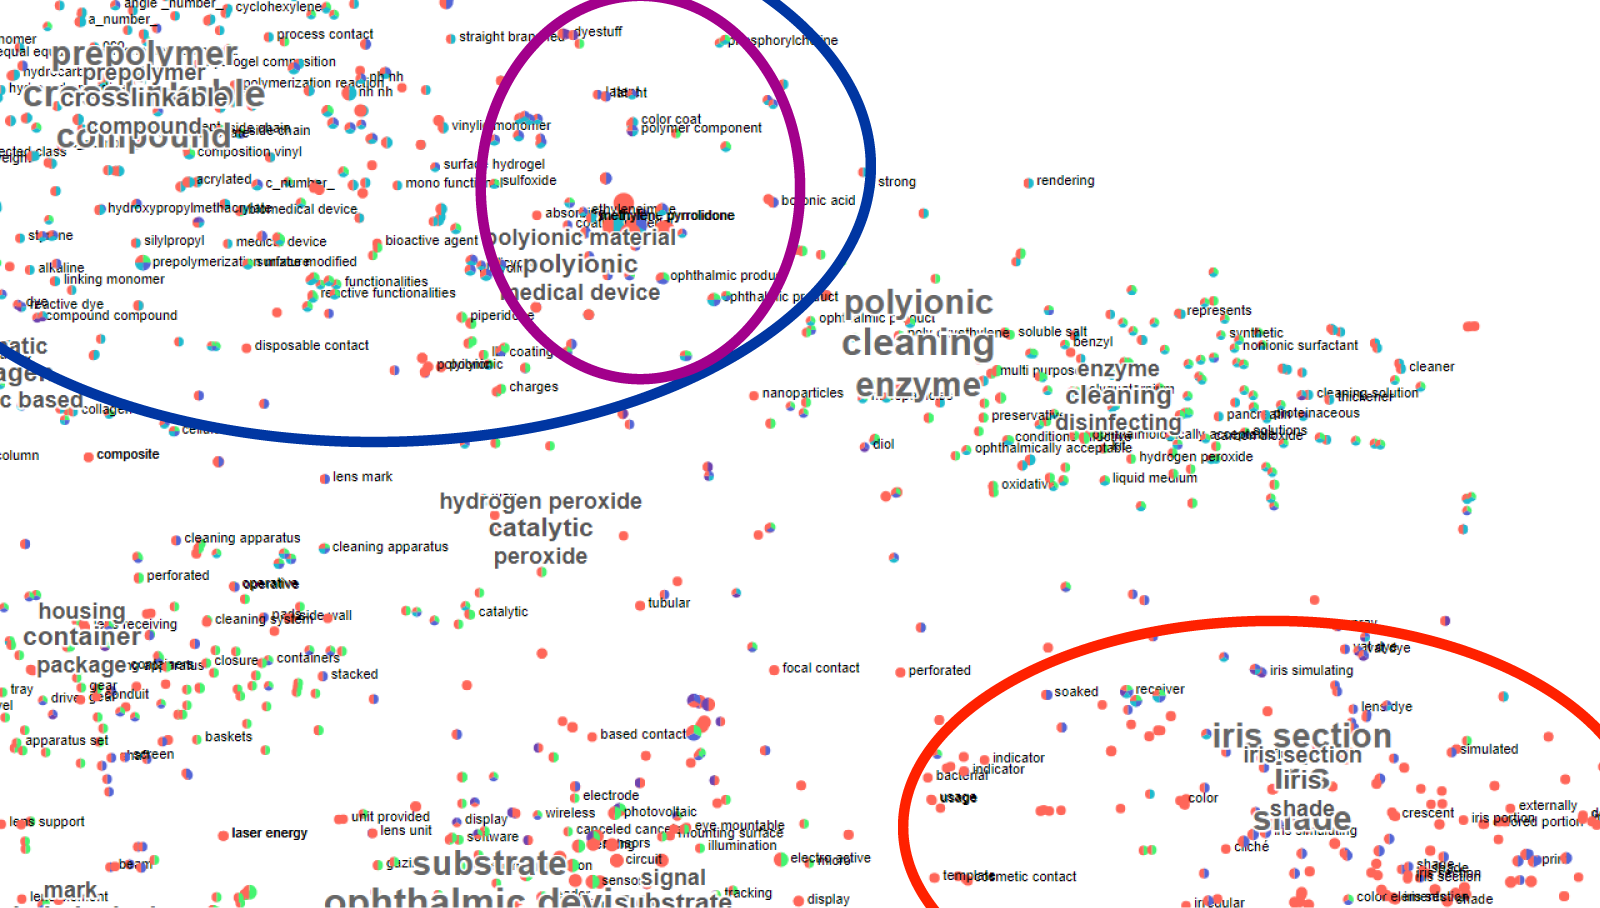
\includegraphics[width=\textwidth]{img/colored_ink_baseline}
        \label{fig:colored_ink_baseline}
    }
    \caption{Areas relevant for task 7. Colored contact lenses (red), materials for making lenses (blue), inks for printing on colored lenses (purple).}
    \label{fig:colored_ink}
\end{figure}

For colored contact lenses, there exists an area focusing on ink for printing on colored contact lenses.
For the semantic approach (see Figure \autoref{fig:colored_ink_semantic}, it lies inside cluster \textnumero3, which specializes on chemical substances for the production of lenses.
The area about ink lies between the ``chemical'' cluster \textnumero3 and the cluster \textnumero6 with colored contact lenses.

For the baseline approach, the cluster \textnumero3 (materials)  and cluster \textnumero6 (colored contact lenses) are situated further away from each other and do not touch directly (see Figure \autoref{fig:colored_ink_semantic}.
Nevertheless, the area about ink is at the edge of cluster \textnumero3 that is closest to cluster \textnumero6 .

\begin{figure}[!]
    \centering
    \subfigure[Semantic approach]
    {
	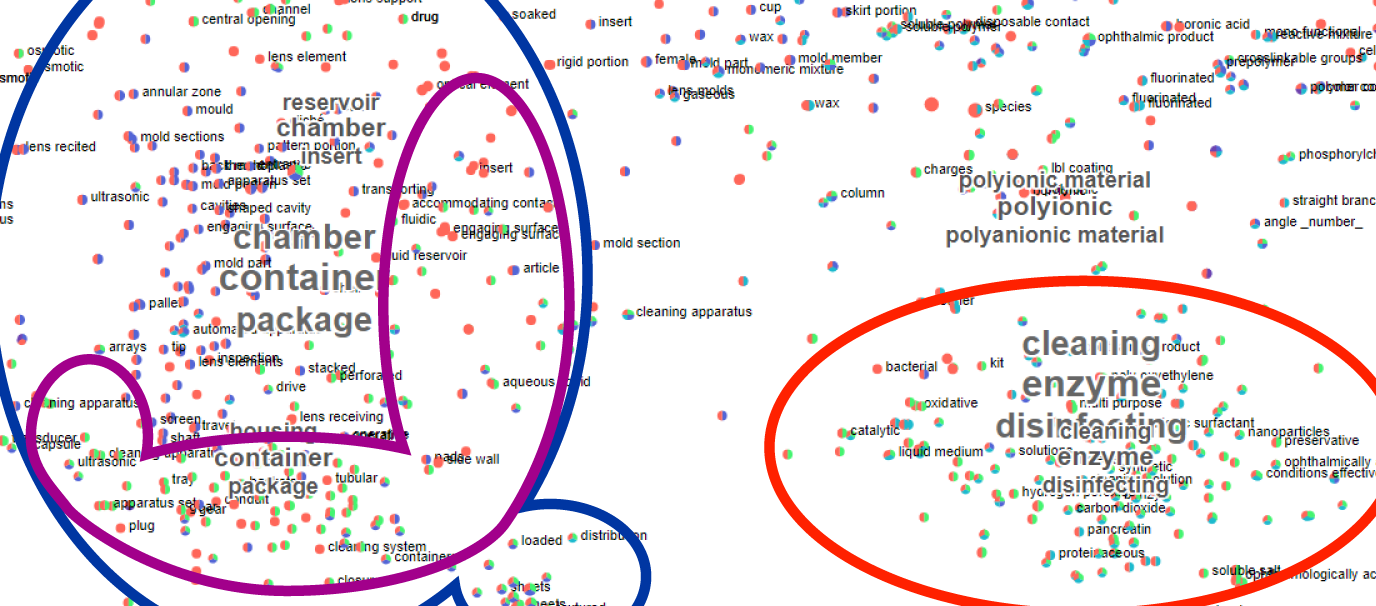
\includegraphics[width=\textwidth]{img/cleaning_package_semantic}
        \label{fig:cleaning_package_semantic}
    }\\
    \subfigure[Baseline approach]
    {
        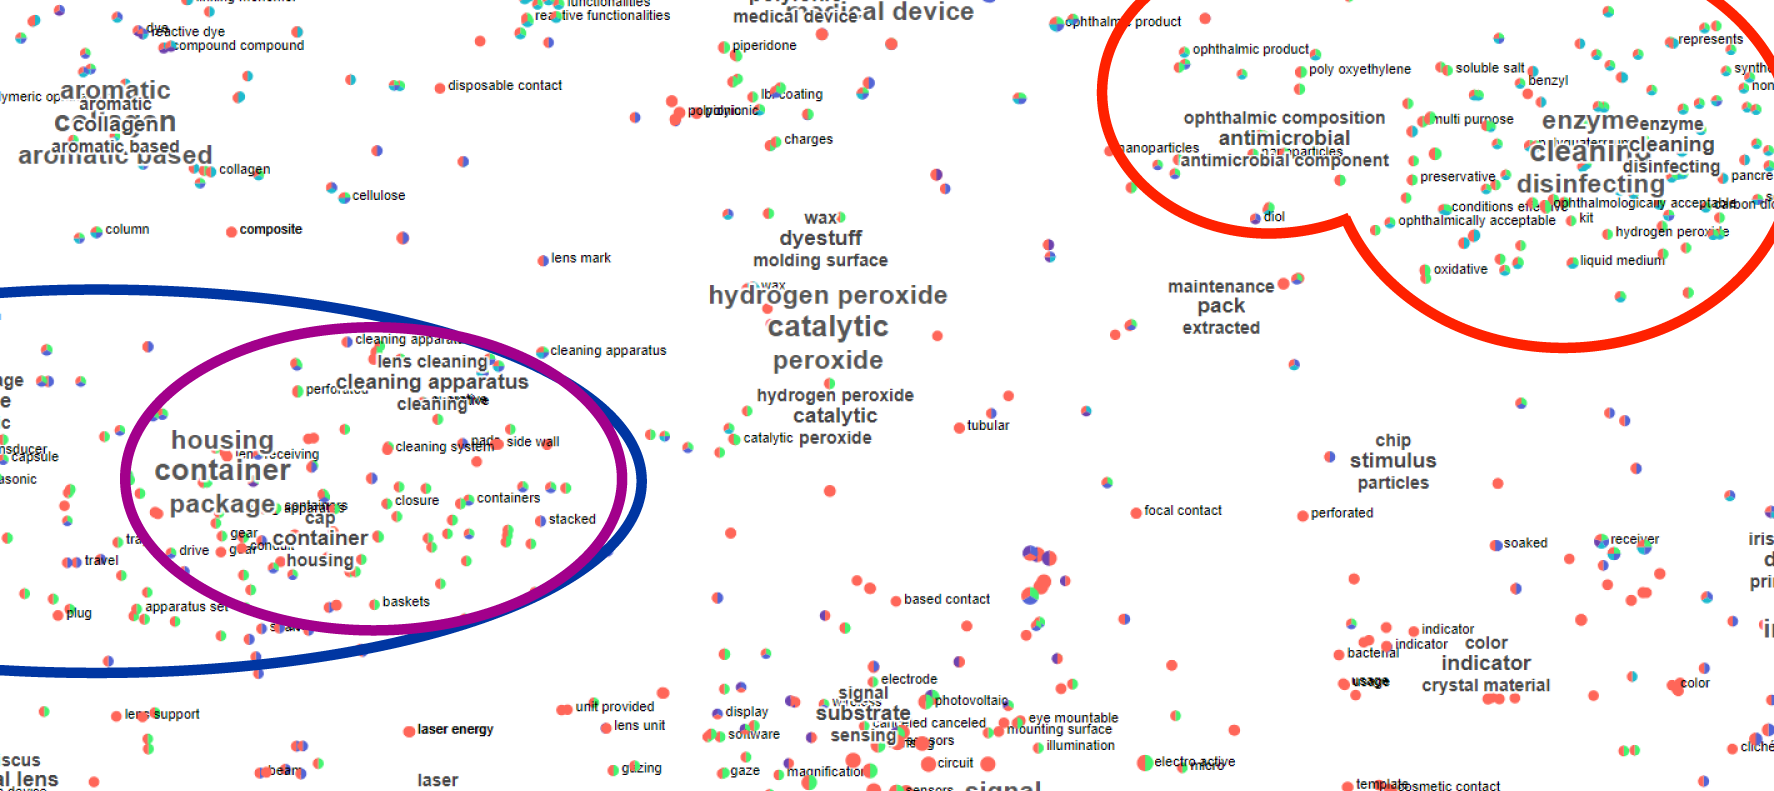
\includegraphics[width=\textwidth]{img/cleaning_package_baseline}
        \label{fig:cleaning_package_baseline}
    }
    \caption{Areas relevant for task 9. Cleaning of contact lenses (red), storage of lenses (blue), containers with cleaning solutions (purple).}
    \label{fig:cleaning_package}
\end{figure}

For cleaning of contact lenses (cluster \textnumero1), a smaller related area is situated inside the cluster \textnumero5 about packaging and storage of lenses.
It is predictable because containers for lenses often include a cleaning solution.
Same as with task 7, the clusters produced by semantic approach are closer to each other (see Figure \autoref{fig:cleaning_package_semantic}.
For the baseline approach, the areas focused on cleaning and packaging are not adjacent (see Figure \autoref{fig:cleaning_package_baseline}).
For both approaches, the area about containers with cleaning solutions is on the edge of cluster \textnumero5 that is closest to cluster \textnumero1.

In other words,  between tasks 7 and 9 the semantic and baseline approaches behaved in a consistent way with regards to the relative placement of clusters.
The semantic approach seems to place areas with strong thematic connections closer to each other.
Notably, no other unrelated patents were situated between the two clusters of interest.
The space between them was either empty or occupied with patents related to both clusters.
This was not the case with the baseline approach, in which unrelated patents occupied the gap.
One possible explanation for this phenomenon might be that the semantic representations result in more ``continuous'' areas where topics ``flow'' into one another.
\gls{tf-idf}-based vectors, on the other hand, might produce more ``interrupted'' or ``discrete'' structures that are more likely to be rearranged during the dimension reduction process.

\subparagraph{Intended solution}~\\
We assumed that the large clusters would be found fairly quickly based on their key terms. 
Then smaller related areas could be discovered by following the citation connections.
The user is supposed to briefly hover over a number of patents within an area they consider definitely relevant.
If most citation lines lead to one particular area outside of the current cluster, then it might be worthwhile to follow them and inspect the other area.

\subparagraph{Summary}~\\
All participants found the requested large clusters for both tasks fairly quickly by reading the key terms for the large clusters.
They then confirmed their assumptions by zooming into the selected cluster and reading terms, or in some cases, titles and abstracts of the patents situated there.

Two experts came up with the idea of using citations to find related areas.
One of them even realized that many connections led to the same spot, but could not interpret this information further: ``Even though with all those lines going to here and there I can see the other areas on the landscape, I still find it difficult to generate knowledge from that''.
This participant by chance examined only cited patents that were not directly thematically related to the region of interest.
It is completely understandable that they could not see a direct connection.
Ultimately, no expert could successfully identify the smaller related areas supplementary to the noticeable large clusters.

\paragraph{Searching for small areas}~\\
Same as with tasks 7 and 9, task 8 and task 10 were intended to be solved in a similar way for comparability.
Here, using the filtering controls was allowed and encouraged.

\subparagraph{Intended solution}~\\
For contact lenses with electronic components, one could safely assume that those patent applications are fairly recent.
After restricting the timeline to the years after 2000, one can observe that the \gls{ipc} class ``H - electricity'' grew in proportion from almost invisible 1.5\% to 2.2\%.
Electricity is a plausible \gls{ipc} section, so after selecting that ``H'' node, there are virtually no documents left except one densely populated spot (see Figures \autoref{fig:electronic_components_semantic} and \autoref{fig:electronic_components_baseline}).
It approximately matches the cluster \textnumero7 with terms \textit{substrate, signal, sensing} (for semantic approach) or \textit{ophthalmic device, substrate, energy} (for baseline approach). 
The user could then try lifting the filters and checking whether the patents inside the area of interest, but from outside of \gls{ipc} class ``H'' and those filed before 2000 are relevant, too.

\begin{figure}[!]
    \centering
    \subfigure[Semantic approach]
    {
	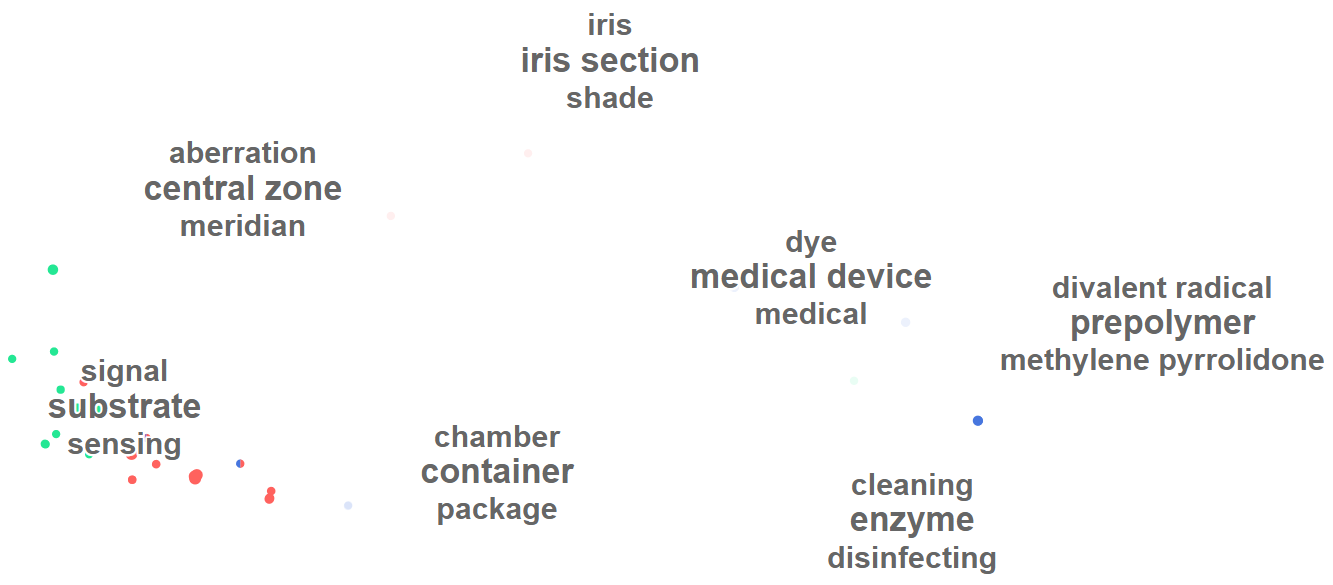
\includegraphics[width=\textwidth]{img/electronic_components_semantic}
        \label{fig:electronic_components_semantic}
    }\\
    \subfigure[Baseline approach]
    {
        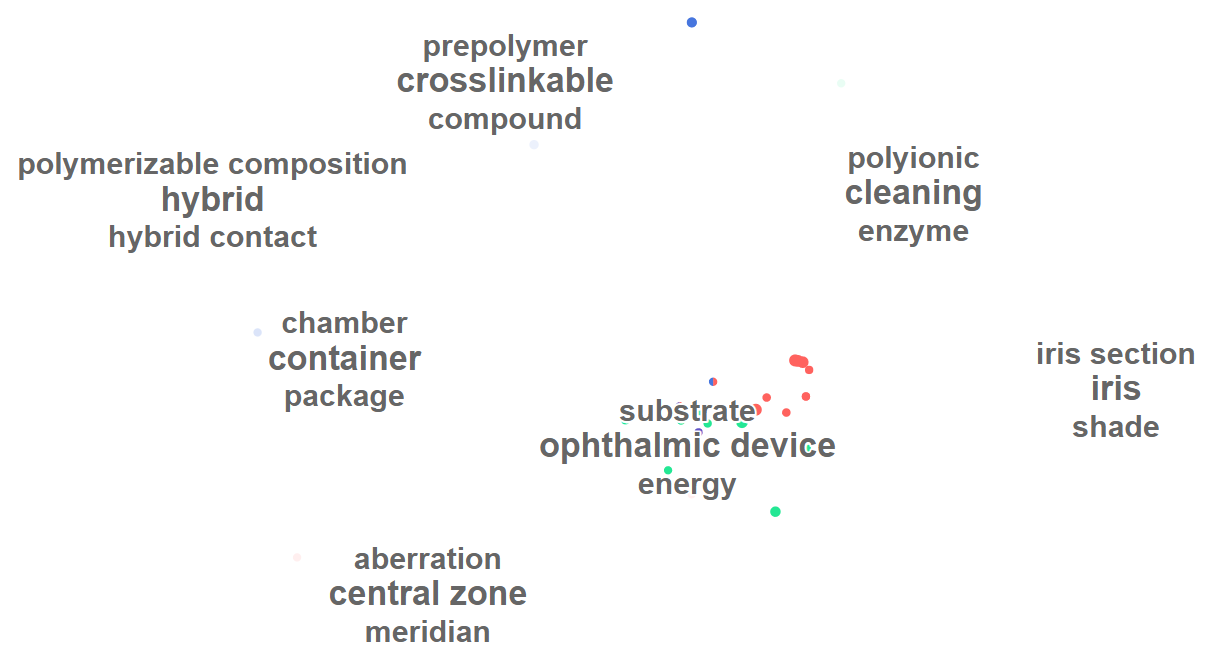
\includegraphics[width=\textwidth]{img/electronic_components_baseline}
	\label{fig:electronic_components_baseline}
    }
    \caption{The landscape as seen after the proposed sequence of actions for solving task 8. The landscape is restricted to years after 2000 and \gls{ipc} class H - ``electricity''.}
    \label{fig:electronic_components}
\end{figure}

Upon further inspection, with the semantic approach it should become clear that approximately one-fourth of cluster \textnumero7's area is mostly dedicated to various industrial automation systems.
Those systems definitely include electronic components, while the lenses itself do not.
The fact that they were grouped together with smart contact lenses was foreseeable and meaningful because of the shared vocabulary.
The remaining three-fourths of the area comprise the intended answer to task 8 (see Figure \autoref{fig:industrial_automation_semantic}).
For the baseline approach, the separation between patents pertaining to automation systems and patents about smart contact lenses is less clear (see Figure \autoref{fig:industrial_automation_baseline}).
The patents irrelevant for this task intersperse cluster \textnumero7.
This is evidence of the superiority of the semantic approach for this particular case.

\begin{figure}[!]
    \centering
    \subfigure[Semantic approach]
    {
        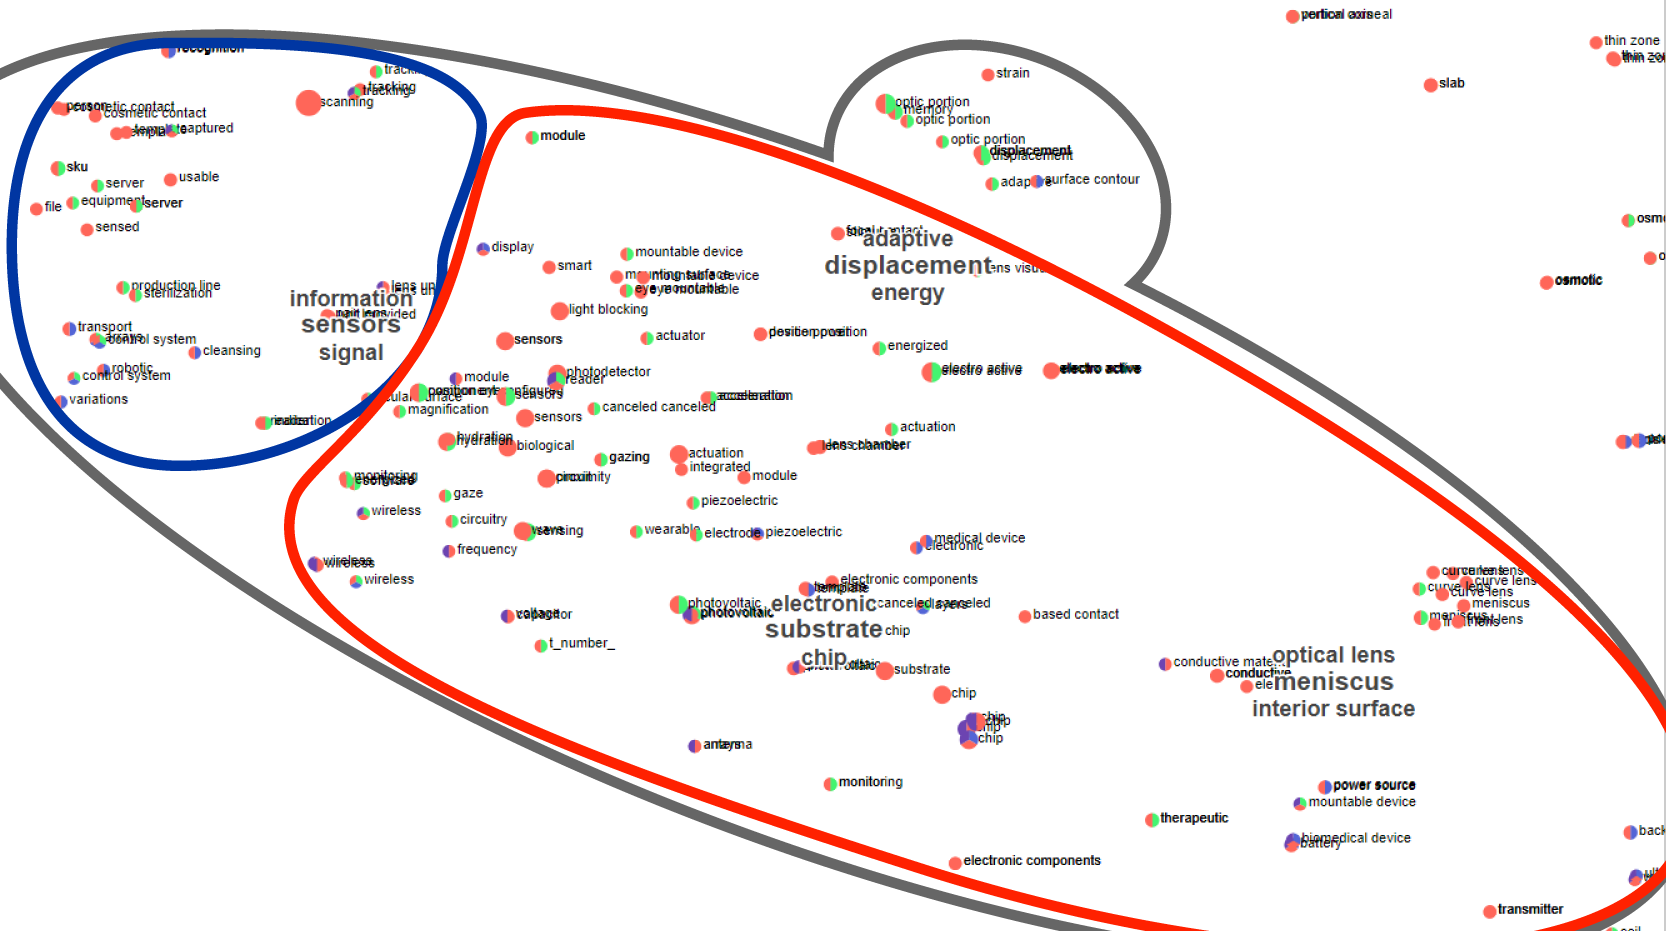
\includegraphics[width=\textwidth]{img/industrial_automation_semantic}
        \label{fig:industrial_automation_semantic}
    }\\
    \subfigure[Baseline approach]
    {
	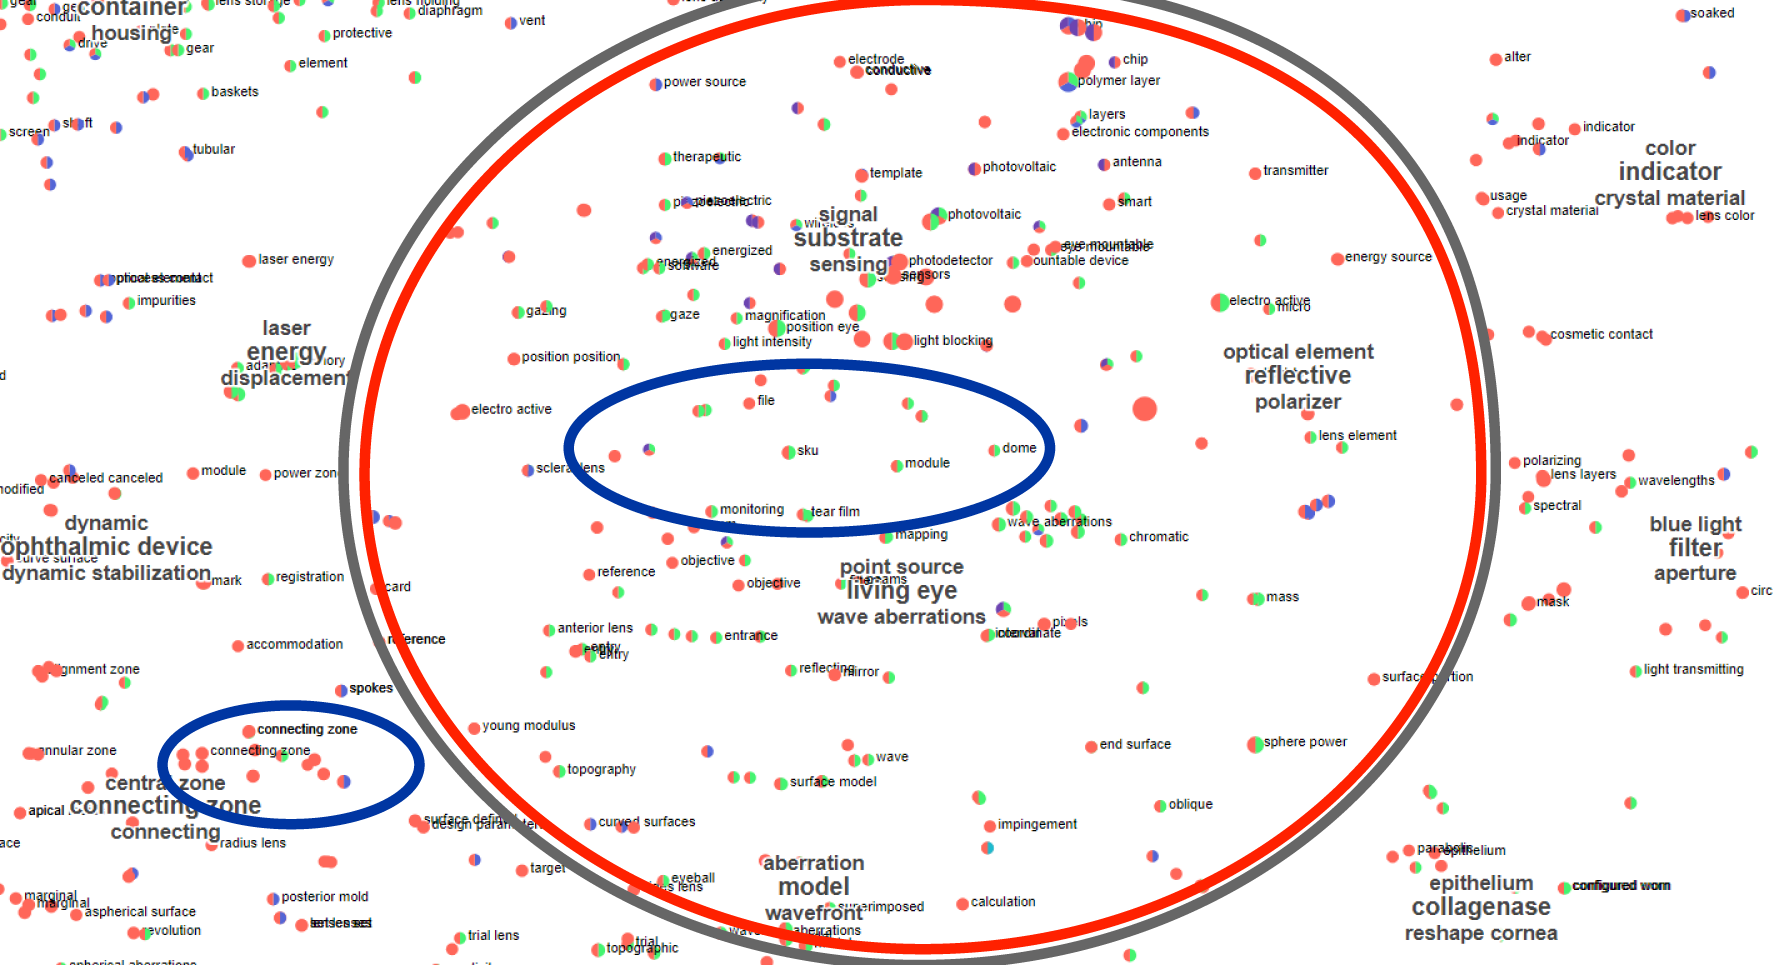
\includegraphics[width=\textwidth]{img/industrial_automation_baseline}
        \label{fig:industrial_automation_baseline}
    }
    \caption{Cluster \textnumero7 as seen in both approaches. The area relevant for task 8 is shown in red, the area about industrial automation systems is shown in blue, the cluster boundaries are shown in gray}
    \label{fig:industrial_automation}
\end{figure}

\subparagraph{Experts' solutions}~\\
The study showed that the intended sequence of steps for solving the task was too complicated, at least for our experimental setting.
None of the participants chose to use any filtering options.
Moreover, the sunburst hierarchy was switched to \textit{country} after the previous task, which resulted in a monochrome view.
No participant wished to switch back to \textit{\gls{ipc} class} for a colorful display.
This might mean that for this task, the participants concentrated exclusively on reading cluster and document terms and did not see a need to involve other controls.
Another explanation is also plausible: as the participants saw a single-colored representation, it did not occur to them to change it because they briefly forgot that it is possible.
Maybe if they had a sunburst hierarchy unsuitable for this task already selected (i. e. \textit{assignee}), they would have noticed the mismatch and would have tried to fix it.

The participants expressed the wish for a search feature because they would rather use it for such kind of task than browse around hoping to stumble upon the right area: ``it's fairly difficult to find the right area if it [what you're looking for] is not labeled in the big regions''.

Ultimately, three experts were able to identify cluster \textnumero7 as the relevant area.
Unfortunately, they did not examine the area thoroughly enough to discover the irrelevant quarter of the documents.
One expert started their search in the ``chemical'' area as they argued that polymers are the basis onto which the electronic components are placed: ``the electronic components should be included in polymer materials somewhere''.
The participant browsed around until they stumbled upon the medium-sized cluster with the terms ``signal, substrate, sensing'', which they recognized as the area of interest.

Two other participants were steered to the correct answer by terms such as ``signal, substrate, sensing'' and ``energy''.
They then confirmed their guess by reading some patent titles.
The one expert who did find a wrong solution to the task was distracted by the plausible, but irrelevant term ``medical device'' in cluster \textnumero3.
Our examination revealed that the term ``device'' in the above-mentioned area is not used to mean ``appliance'', but refers to the lens itself as a product for medical purposes.

\todo{task 10}

\paragraph{Relative positions of clusters}~\\
For the semantic approach, one participant said ``there are distinctly separated areas, it can be clearly seen''.
Another expert noted that ``areas are separated more clearly'' in the semantic approach, and that it looked ``less noisy and more focused''.
Both of them also remarked that the clusters related to the chemical composition of contact lenses (see clusters \textnumero2 and \textnumero3 from \autoref{tab:comparison_clusters}) are supposed to be situated close to each other: ``I think those two belong together''.
One participant also noticed a difference in this area between the two approaches: ``the polymer stuff was in two areas before and now it is in only one'' (in this case, ``before'' refers to the baseline approach and ``now''  to the semantic approach).

\paragraph{Summary}~\\
Ultimately, the semantic approach seemed to reflect the structure of the domain in a better way.
This, however, did not influence the experts' strategy much, as the overall structure of the clusters was comparable.
The proposed visualization approach itself mattered more than the method for placing the data points.
When it comes to the specific tasks we offered, the hypothesis is likely to be confirmed.

\paragraph{Limitations of qualitative evaluation}~\\
It is important to note that the tasks created for the study cannot possibly evaluate the distances between the documents as a whole.
When it comes to subjective perception, we can only witness the experts' mental processes and their opinions.
We can merely capture a small sample due to the limited number of tasks.
A quantitative evaluation would be necessary to evaluate the placement of documents as a whole.
%This led us to propose another, objective way to evaluate how distances express similarity in a given dataset.
%We argue that distances in the visualization space between patents and their citations are a suitable indicator of similarity because citations constitute prior art, which means a certain degree of relatedness.
%Admittedly, not every citation is absolutely relevant to the newer patent, however, we assume that citations as a whole represent similarity sufficiently well.
%To obtain a measure of quality for some configuration of points in the visualization space, one needs to consider all pairwise distances 

\subsection{\gls{sus}}
\label{subsec:sus}

A German translation \cite{Rauer2011} of a \gls{sus} questionnaire was used after the first part of the study. The prototype received an average \gls{sus} score of 68.12 points, with a negligible difference of only one point between two tested approaches. It is important to remember that the \gls{sus} score is not a percentage, so it is necessary to consider the percentile when interpreting the value. According to \cite{Bangor2009}, an application is considered ``acceptable'' at around 68-70 \gls{sus} points, which is also the average.

When participants explained their answers, they mostly named the technical imperfections of the prototype as reasons for lower scores. 
The performance on the contact lens dataset with about 2500 data points was not optimal and resulted in processing delays of up to two seconds, especially when hovering and clicking on the sunburst. 
It was important for us to provide an extensive dataset with sufficient thematic variation, so we willingly accepted the delays for that reason.
The performance of the prototype was mentioned by the users: ``I would use it, assuming it runs faster'', ``The operation is not cumbersome, but difficult because of the delay. Because it is so simple, it should run smoothly''.

The experts confirmed that the prototype was easy to use: ``It is easy because there are not infinitely many options to click on'', ``I didn't find it excessively difficult to use'', ``It would not take long to train someone to use it''.
They also missed features that one would expect from a finished piece of software: ``What is implemented is coherent and conclusive, you could extend it nicely'', ``It does not exploit all possibilities''.

While we are not proposing a commercially viable software product, we are conscious of the fact that it is difficult for users to evaluate prototypes with a limited number of features. 
Users are usually confronted with commercial software and therefore expect a comparable amount of development effort from every piece of software they encounter.
Considering all of the above, we view the ``average'' \gls{sus} score as a success.

\subsection{Questionnaire for comparing the approaches and the following mini-interview}
\label{subsec:questionnaire_comparing_approaches}

If we consider differences in the answers between two approaches, they comprised 31\% on average.
69\% of the answers were identical for the same participant.

One participant felt that the baseline approach was ``a bit better'', but was not able to explain why.
Other participants did not see a significant difference between the two approaches: ``I am unable to say whether one or the other is better'', ``maybe I contradict myself [in the answers] compared to the other one, they are not that different''.

All participants saw value in the proposed visualization approach as a whole, independently of the kind of document embeddings which is used.
They emphasized that it is an easy way to get a general idea about the domain one is dealing with: ``It is a fast possibility to be able to say what areas you are working with'', ``the topics are prepared how one would expect them to be''.
The expert compared the visual approach to patent landscaping with existing commercial solutions: ``In other tools you can do an \gls{ipc} analysis. This here is another approach with the same goal''.
They emphasized that with our proposed approach one must not heavily rely on knowledge of \gls{ipc} classes.

One expert stated that ``you can discover connections [with the prototype]''.
They expect that the prototype ``can provide benefits in industry and research''.

\section{Discussion}
\label{sec:discussion}

\subsection{The visualization approach and interaction metaphors}

The prototype received an average SUS score which is considered acceptable, even though it lacked some features the participants expected or wished for.
Their wishes were undoubtedly at least partly shaped by the participants' prior exposure to the patent landscaping tool STN Anavist, which is a commercial product and therefore cannot constitute a fair comparison to our proof-of-concept prototype.
Overall, the participants' impression of the prototype was positive and they confirmed the need for such a tool.

Several relatively minor usability problems had been uncovered during the evaluation.
First, panning and zooming start to noticeably lag when working with over 2000 patents, which resulted in performance problems. 
This was an inconvenience to the experts and affected their understanding of the current state of the sunburst.
Another usability issue that the participants remarked on were data points situated close to each other so that the labels overlap making the terms per patent unreadable.

Overall, the chosen visualization metaphors fit the task and were understood by the participants.
The heuristic for the dynamic label density successfully provides a balance between text and whitespace.
The dynamic mapping of colors depending on the state of the sunburst and glyphs as indicators of co-occurrence were quickly grasped by the participants.
Just as well did the participants understand how the interconnected views affect each other's states.
Considering the very short training the participants received, our visualization approach proved to be intuitive.

Thinking back to the research questions defined in the case study, we successfully found interactions techniques that are able to combine metadata of various types and semantic dimensions.
The semantic space adds a dimension where one can find patterns via distributions of values of metadata attributes.
For example, colors of the points likely contributed to the participants' perceptions of clusters.

The proposed visualization approach provides added value for various patent landscaping scenarios such as technology trend analysis\todo{etc}.
At the same time, there are no restrictions that would speak against the use of our approach for any kind of text documents characterized by metadata, for example, scientific publications.

The benefits of our proposed approach are especially evident when a brief overview of various thematic areas in the dataset is necessary.
Detailed queries are better fulfilled using conventional tools such as textual search, bar charts and co-occurrence matrices.

\subsection{Semantic embeddings versus TF-IDF embeddings}

The think-aloud study resulted in inconclusive data with regards to the comparison of the two approaches.
It has been shown that the approach itself only played a minor role in the evaluation process.
The task-solving process was significantly more influenced by the interface of the visualization and its features.

According to some participants, the semantic embeddings resulted in a more intuitive relative placement of clusters.
The clusters in the semantic approach were also separated in a better way according to our own examination and participants' perceptions.
This might be attributed to the fact that semantic embeddings are dependent on the context of a word and therefore better capture similarities for synonyms, hypernyms, words used often in similar sentences, etc.
However, the tasks we designed for the study could only possibly evaluate a subset of the documents with regard to their relative placement.
Only a quantitative approach would be able to assess the positions of patents in visualization space as a whole.
It is therefore impossible to draw a definitive conclusion at this point.